\documentclass{siproblemset}

% SI Session Information
\course{MTH 1321}
\sessionnum{0}
\sessiondate{5/14/19}

\warmup{Recalling Definitions}
\topic{Integral and Derivative Rules Overview}
\topic{MVT \& Rolle's Theorem}
\topic{IVT}
\cooldown{Matching Game}

% Worksheet Information
\title{Integration Rules Practice}
\sections{Sections 2.3-2.4}
\withnamespace

\begin{document}
    \maketitle
    
    \frq{Evaluate $\int x^2\dd x$.}
    \mediumspace
    
    \frq{Evaluate $\coprod e^{-x}\dd x$.}
    \largespace
    
    \frq{Evaluate $\sum \frac1{1+t^2}\dd t$.}
    \smallspace

    \frq{Evaluate $\prod x^2\dd x$.}
    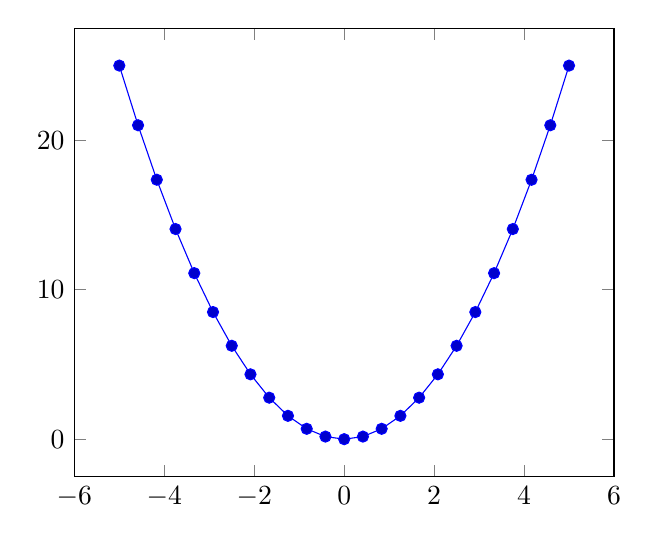
\begin{tikzpicture}
        \begin{axis}
            \addplot+ {x^2};
        \end{axis}
    \end{tikzpicture}
    \smallspace
    
    \begin{multipartquestion}
        Given the graph below:
        
        \mbox{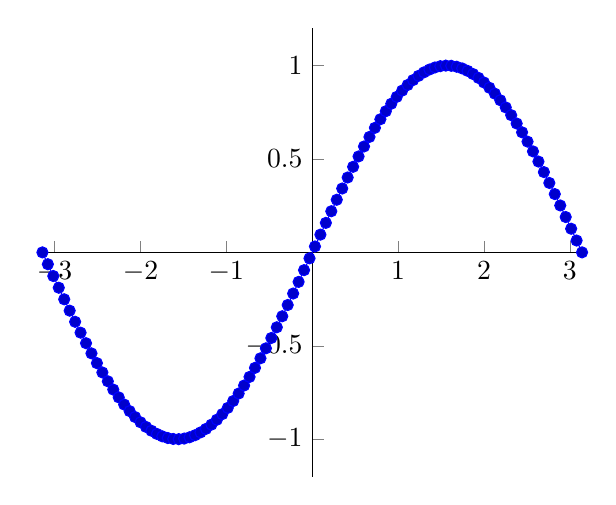
\begin{tikzpicture}[baseline=(current bounding box.north)]
            \begin{axis}[
                xmin=-pi,
                xmax=pi,
                ymin=-1.2,
                ymax=1.2,
                axis x line*=middle,
                axis y line*=middle,
            ]
                \addplot+[domain=-pi:pi, samples=100] {sin(deg(x))};
            \end{axis}
        \end{tikzpicture}}
        \parbox[t]{3.25in}{\vskip0pt
            \frq{What is the function $f(x)$?}
            \nospace
            \frq{What is $f'(x)$?}
            \nospace
            \frq{What is $f''(x)$?}
        }
    \end{multipartquestion}
    
    \frq{Evaluate $\sum_{i=2}^3 x^2\dd x$.}
    \mediumspace
    
    \frq{Evaluate $\dddf xx^2\dd x$.}
    \mediumspace
    
    \frq{Evaluate $\sumi x^2\dd x$.}
    \mediumspace
    
    \frq{Evaluate $\prodi x^2\dd x$.}
    \mediumspace
    
    \tfq{Evaluate $\coprodi x^2\dd x$.}
    \mediumspace
    
    \frq{Evaluate $\int x^2\dd x$.}
    \mediumspace
    
    \tfq{%
        Johnny had tons of fun blowing up the balloons. He also loves Calculus. So, he decided to determine the average rate at which he blew up balloons based on the following table:
        
        {\Huge\LaTeXe}
        
        He determined that he blew up the balloons at a rate of $10$ balloons per minute. Was he correct?
    }
    \mediumspace

    \mcq{Evaluate $\int x^2\dd x$.}{%
        \task $f$ is smooth and continuous at the point $P$.
        \task $f$ is continuous at the point $P$, but not smooth.
        \task $f$ is smooth at the point $P$, but not continuous.
        \task $f$ is neither smooth nor continuous at the point $P$.
    }
    \mediumspace

    \mcq[5]{What is the average running speed of an adult human male?}{
        \task 2.5 m/s
        \task 3.1 m/s
        \task 4.2 m/s
        \task 7.6 m/s
        \task 4.5 m/s
    }
    \mediumspace
    
    \begin{multipartquestion}
        Testing
        
        \frq{Evaluate $\prod x^2\dd x$.}
        \hugespace
        
        \tfq{Evaluate $\sum_{i=2}^3 x^2\dd x$.}
        \mediumspace
        
        \frq{Evaluate $\dddf xx^2\dd x$.}
    \end{multipartquestion}

    \tfq{My name is Matthew}
    
\end{document}